
%---------------------------------------%
% Packages arranged by : Tsz Timmy Chan %
%                 Date : Dec 12th, 2019 % 
%---------------------------------------%

\documentclass{LSRIarticle}
\usepackage{LSRIcommon}

%allows for the use of affiliation
\usepackage[affil-it]{authblk}
\title{Learning Sciences Reading Log}	% Work Title Here.
\author{Tsz Timmy Chan}	% YOUR NAME HERE 



\date{\today}
\usepackage[log]{LSRIheader}


\affil{Learning Sciences Research Institute \\ University of Illinois at Chicago}

\usepackage{setspace}
%\linespread{2}

% Make subsection "Week 1, etc"
\usepackage[explicit]{titlesec}
\titleformat{\subsection}{\normalfont\large\bfseries}{}{0em}{#1: Week\ \thesubsection}
\renewcommand{\thesubsection}{\arabic{subsection}}


% make it so there's no indent
\setlength{\parindent}{0pt} 


\addbibresource{My_Library.bib}		% Reference file, NO SPACES in the name
\input{TCglossary}					% Glossary file for acrynoms and whatnot


\begin{document}
%\smalltitle


\clearpage\maketitle
\thispagestyle{empty}

\section*{Introduction}

%---------------------------------------%
% Packages arranged by : Tsz Timmy Chan %
%                 Date : May 26th, 2019 % 
%---------------------------------------%

\documentclass{TC}
\usepackage{TCcommon}

\title{TITLE HERE}	% Work Title Here.
\author{Tsz Timmy Chan}	% YOUR NAME HERE 

\usepackage[notes]{TCheader}
\usepackage{TCexamtitle}

\usepackage{setspace}
\linespread{1.5}

%\renewcommand{\benediction}{" " - }
%\renewcommand{\quoteoftheday}{" " \\ - }

\begin{document}
This collection of notes from readings and class discussions was first constructed using \LaTeX\; in the Fall semester of 2019. The Notes and Glossary files organize and chronicle the thoughts and summaries from the reading involved in this program. 
\end{document}

\newpage
\tableofcontents
\newpage
\listoffigures

\newpage

\setcounter{section}{-1}
\section{Summer 2019}

%---------------------------------------%
% Packages arranged by : Tsz Timmy Chan %
%                 Date : May 26th, 2019 % 
%---------------------------------------%

\documentclass{TC}
\usepackage{TCcommon}

\title{TITLE HERE}	% Work Title Here.
\author{Tsz Timmy Chan}	% YOUR NAME HERE 

\usepackage[notes]{TCheader}
\usepackage{TCexamtitle}

\usepackage{setspace}
\linespread{1.5}
\usepackage[acronym]{glossaries}

\makeglossaries
%\renewcommand{\benediction}{" " - }
%\renewcommand{\quoteoftheday}{" " \\ - }

\begin{document}

Math and Science Education Journal Club
\begin{itemize}
\item The group and I read about \gls{ltp}, and we differentiated \gls{ltp}, where trajectories are for mathematics, and progression is for science
 \parencite{duncan_learning_2018, schwarz_developing_2009, lobato_taxonomy_2017}. 
\item Role of neuro in learning sciences \parencite{jacobson_conceptualizing_2016}.
\item The group read about gender and identity in learning \parencite{darragh_identity_2016, liben_developmental_2014}.
\item The group and I read about maker spaces \parencite{halverson_maker_2018, blikstein_assessment_2017}.
\item The group and I read about transfer of math knowledge into sciences \parencite{britton_case_2005, roberts_index_2007, tariq_defining_2008}.

\end{itemize}
\subsection{Learning Trajectories and Progressions}
Very initial thoughts on Learning Trajectories: 

%
%--------------------------------------------%
% Packages arranged by : Tsz Timmy Chan	     %
%                 Date : June 12th, 2019     %
%--------------------------------------------%

\documentclass{TC}
\usepackage{TCcommon}

\title{Learning Trajectories and Progressions}	% Work Title Here.
\author{Tsz Timmy Chan}	% YOUR NAME HERE 


\usepackage[style=numeric]{biblatex}
\addbibresource{LS.bib}


\usepackage[notes]{TCheader}
\usepackage{TCexamtitle}
%\renewcommand{\benediction}{" " - }
%\renewcommand{\quoteoftheday}{" " \\ - }
\begin{document}
\subsubsection{Learning Trajectories and Progressions}
In order to give a proper definition of learning trajectories and progressions, we must first begin with preliminary definitions.

Given an academic discipline, there exist ways to describe the paths to student growth and mastery. Researchers and teachers conduct this theoretical work with variety of intentions and focus, leading to a corniucopia of styles and approaches to the study and creation of learning trajectories and progressions. In  \parencite{duncan_learning_2018}, Duncan and Rivet give a general definition of \gls{ltp}. In \parencite{lobato_taxonomy_2017}, Lobato and Walters give a detailed description of seven different types of intentions/perspective on \gls{ltp}. 
 
First, knowledge in an academic field beckons organization, and the first operation we do is to separate out knowledge into \emph{constructs}, which are defined as follows:

\begin{mdframed}
\begin{definition}[Construct]
\emph{Constructs} are large ideas in an academic discipline, usually defined in a way to partition a subject in order to understand cognition and learning. One can consider this defining subsets of the knowledge of a discipline.  \end{definition}
\end{mdframed}

Note that constructs are subjectively defined, and the ways they are defined reveal the researcher's intention. Furthermore, constructs may contain other constructs; I.e., If $A$ is some construct, then there may exist $A_1, A_2, \ldots, A_n \subset A$. Note that in this description, we consider finite $n$, as most applications of hypothetical models of learning in the form \gls{ltp} contain finitely many constructs.

\begin{example}
Suppose we have a topic $A = \text{"Functions in Precalculus"}$, and we wish to use a disciplinary-logic approach (defined in \ref{disciplinary_logic}) to describe a set of constructs that may be defined using skills and definitions. For a rudimentary example:
\begin{align*}
A_1 &= \text{"Use of variables"},\;A_2 = \text{"Mapping / Relations"},\\
A_3 &= \text{"Graphs of equations in } \R^2 \text{"},\;A_4 = \text{"One to one"},\\
A_5 &= \text{"Inverse functions"}, \cdots \\
\text{by construction: }& A_1, \cdots, A_5 \subset A
\end{align*} 
\end{example}
Note here that for some arbitrary $i,j$, $A_i \cap A_j \stackrel{?}{=} \emptyset$. 
\begin{mdframed}
\begin{definition}[Pathway between constructs]
A pathway between constructs shows a connection between ideas, usually for pedagogical reasons or disciplinary expertise. A pathway between constructs may contain intermediate steps, with a diverse set of pathways. 
\end{definition}
\end{mdframed}

\begin{remark}
I wonder if creating \gls{ltp} with disjoint constructs is useful or not? Or acknowledging the overlaps can create better "knowledge webs"? Can one define the pathways and the constructs the edges and nodes of knowledge countable? discrete?
\end{remark}
 
 In essence, once constructs are separated out and defined using some rule (this may be based on education research or academic expertise), one is imposing some partial order on these constructs, where the this order may be defined in multiple ways, depending on the academic field.
 
 \begin{mdframed}
\begin{definition}[Learning trajectories and progression]
A \emph{learning trajectory} (LT) or \emph{learning progression} (LP) is a hypothetical model used describe student growth and mastery in an academic subject, usually with intermediate \emph{levels} and \emph{pathways}. Usually, mathematics educators use "trajectories" and science educators use "progressions". We call a \gls{ltp} \emph{linear} when the \gls{ltp} models a \emph{well ordered set}.
\end{definition}
\end{mdframed}
\subsubsection{Common Properties of \gls{ltp}}

As researchers have finite time and resources, one must define a limitation on the scope of an \gls{ltp}:

\begin{mdframed}
\begin{definition}[Scope of \gls{ltp}]
\gls{ltp} have a defined \emph{scope}, which consists of
\begin{itemize}
\item a particular slice of knowledge (domain of study), \item and a specific age-group (span).
\end{itemize}
Conventionally, the starting point of an \gls{ltp} is called the \emph{lower anchor}, represented with a beginner or novice level of understanding within the scope, and the ending point of an \gls{ltp} is called the \emph{upper anchor}, which represents the proficiency level within the scope.
\end{definition}
\end{mdframed}
\gls{ltp}, by its nature, describe student mastery and progress over a given scope. Naturally, this gives rise to another component of \gls{ltp}:
\begin{mdframed}
\begin{definition}[Levels of \gls{ltp}]
A \gls{ltp} usually contain definitions of levels, which are types of construct that are categorized by \parencite{duncan_learning_2018} \parencite{lobato_taxonomy_2017}:
\begin{enumerate}[(i)]
\item Content ideas or cognative conceptions, \label{levels_content}
\item Practice and discourse patterns \label{levels_practice_and_discourse}
\item A mix of \ref{levels_content} and \ref{levels_practice_and_discourse} 
\item Observable strategies
\item Textbook tasks
\end{enumerate}
\end{definition}
\end{mdframed}

A way to study and compare two different \gls{ltp} in the same field is to consider how many constructs are spread over a particular length of time. This gives rise to the following definition:

\begin{mdframed}
\begin{definition}[Grain Size of \gls{ltp}]
The "size" of the jump between each level or construct. Usually can be viewed the following: Let $c$ be the number of constructs, and $t$ be the amount of time in the scope of the LT. Then the grain size is defined as $g = \displaystyle \frac{c}{t}$. Furthermore, given $g_1 , g_2$ are two grain sizes, suppose $g_1 < g_2$, then we say $g_1$ is "coarser" and $g_2$ is "finer". (This is the same language as the descriptors for the partition of an interval.)
\end{definition}
\end{mdframed}
 \begin{remark}The grain-size and the number of paths given differ based on the intention of the researcher as well as the targeted audience.  \end{remark}

Given that \gls{ltp} describe "growth", this implies that there is some order that can be imposed on the models of student mastery over knowledge, either in terms of content, dialogue or both. Thus, the language of partially ordered sets is appropriate here, where each level or construct is an element, and the pathways between the levels is an edge or order relation. Thus \gls{ltp} may be considered as a directed graph. 

Since \gls{ltp} describe growth from point $A$ to point $B$, we may impose an \emph{order} on the set of knowledge, once constructs and levels are defined. Some common types of ways to characterize and measure "progress" \parencite{duncan_learning_2018}: 
\begin{mdframed}
\begin{definition}[Individual progress along a \gls{ltp}]
Individual progress can be defined as "major re-conceptualizations of knowledge and beliefs because students' na\"ive understandings are often incommensurate with canonical scientific ideas." - Idea is that students have a network of knowledge that becomes better approximations of the expert knowledge as students progress along the levels.
\end{definition}
\end{mdframed}

Individual progress has been the center of study for most subjects, while in mathematics education there's been another perspective on viewing progress:

\begin{mdframed}
\begin{definition}[Community progress along a \gls{ltp}]
Communal progress can be measured as changes in the discourse and practice from the community perspective. Duncan cites Cobb and colleagues \gls{ltp}, which "captures the changes in classroom norms and mathematical practices." Tasks and tools to help achieve the goal of community learning are often included. 
\end{definition}
\end{mdframed}
\begin{remark}
Given a particular discipline, (the pure mathematician in me asks) can we partition a given scope into infinitely many levels, with \gls{ltp} that has infinitely-fine grain size? Perhaps this is the difficulty;t we're using discrete abstractions that hope to closely model the learning process from the instructor or the student perspective, while the experience of learning is one of flow and students experience learning as a continuum of experiences.
\end{remark}

\subsubsection{Claims about \gls{ltp}}
While the constructs is connected to many paths, there seems to be a boundary in which these paths can be drawn effectively. While the number of paths may be infinite, the area which they cover are not. Effective models of descriptive paths is an optimization problem, where there exists finite amount of space and time to describe paths between constructs; and at best, we have some hypothetical model to describe the space of paths between two constructs. These educated conjectures based on research that must be continued to be refined.

\begin{conjecture}[Directed graph conceptualization of \gls{ltp}]
Suppose we impose some order (type of progression) and define constructs associated with the order. Then suppose $A<B$ in some \gls{ltp}. First, there exists at least one path between $A$ and $B$, and there \emph{likely} exists intermediate constructs or levels $\{C_1, C_2, \cdots, C_k\}$. We then define the vertex set to be $\{A, B, C_1, \ldots,C_k\}$ and edges as the pathways between these constructs. This give rise to finitely many paths due to the constraints described above. 
\end{conjecture}

\begin{remark}
Math nerd side note: An \gls{ltp} with this must be some sub-graph of the complete $(k+2)$-directed-graph. This means that the number of pathways, or edges, in an \gls{ltp} with $k$ constructs connecting $A$ and $B$ has the following bounds:

$$ k+ 1 < \text{(Number of pathways)} < 2\sum_{n=0}^{k+1}n = (k+1)(k+2)$$ 

\end{remark}

This way of describing \gls{ltp} gives rise to two quick corollaries:

\begin{corollary}
 \gls{ltp} are not necessarily linear.
\begin{proof}Given we use the language of posets and directed graphs, this is a linear \gls{ltp} is a special case of the general \gls{ltp}. Literature review reveals that "learning is multi-dimensional, context-dependent and therefore likely not linear" \parencite{duncan_learning_2018}\end{proof}
\end{corollary}

\begin{corollary}
A \gls{ltp} may contain cycles.

\begin{proof}In these models, we have directed graphs to indicate progress in maturity of dialogue or to record technical dependencies. Then note that the directed graph that models a particular \gls{ltp} may contain cycles. Duncan and Rivet \parencite{duncan_learning_2018} referred to Battista's research, that students may use more rudimentary ways of reasoning when tackling more complex questions, even though they may have shown proficiency in more sophisticated techniques.
%TODO cite Battista%
 \end{proof}
\end{corollary}
\subsubsection{Development and Refinement of \gls{ltp}}
\gls{ltp} are by definition hypothetical constructs, and their development involves a few usual phases, similar to the engineering design cycle:

\begin{enumerate}[(1)]
\item\label{lit_review} A well formed hypothesis usually begins with a throughout literature review: 
	\begin{enumerate} 
	\item if \ref{lit_review} yields sufficient existing research: design a well-specified \gls{ltp} and go to refinement.
	\item else, use these following techniques \parencite{duncan_learning_2018}:
		\begin{itemize}
		\item Assessment-driven cross-sectional studies of student thinking using interviews and written assessments.
			\begin{itemize}
			\item[Pro:] When interviews are done under status quo setting, the study has the benefit of reflecting what students can do under less than ideal learning environments. Written-assessments\footnote{Commonly used statistical models: Rasch models, latent class analyses, Bayesian networks)} are used to help scale to larger sample of students.
			\item[Con:] Written assessments are difficult to design, especially to elicit responses that can demonstrate the full range of the progression. Optimization problem between the number of assessments and the discrete nature of assessments in a continuum of learning.
			\end{itemize}
		\item short and long (i.e., longitudinal) teaching experiments using design-based research to characterize the development of students' ideas under specified instructional conditions
			\begin{itemize}
			\item[Pro:] Development of instructional interventions modified based on observed student performance allows for a more grass-roots, bottom up approach to validating \gls{ltp}. 
			\item[Con:] \gls{ltp} that is written and designed for a specific condition leads to a question of whether generalizing this is easy. \textbf{Open research question:} Whether learning paths would look different under dissimilar instructional conditions is unknown.
			\end{itemize}
		\end{itemize}
	\end{enumerate}
\end{enumerate}

\subsubsection{Seven approaches to \gls{ltp}}
Lobato and Walters \parencite{lobato_taxonomy_2017} gave a detailed taxonomy of approaches to \gls{ltp} in state-of-the-art research. In their taxonomy, they classify the different approaches into seven categories; however, note that a given \gls{ltp} may be born of a melange of a few perspectives.

\subsubsection{Cognitive levels}

In the cognitive levels perspective, cognitive milestones are ranked in order of sophistication but hierarchies may be weak or strong. Similar to the language used in mathematical induction, strong assumes all steps before are mastered. Mostly linear in nature, but students may enter at a variety of levels and may fall back or climb forward. 
\begin{multicols}{2}
\begin{itemize}
\item Features: Levels or constructs may be organized using mental actions, fine-grained progression or clustering meanings by observing different types of abstraction. For \gls{ltp} written in this approach, emphasis is placed on the quality of the narrative, or group discussions rather than the content.

\item Methods: Created using cross-sectional interviews over multiple grade levels. 

\item Purpose: Diagnostic assessment

\item Benefits: In the example cited by Lobato and Walters, Teachers can access reports of their students' thinking, given that assessments are written to associate particular responses with facets, giving rise to facet-driven instructional resources.

\item Trade-offs: Learning mechanisms on how students morph their understanding by shaping their thoughts from one level to the next is hidden. Progression of understanding of innovative teaching techniques is limited. Important scientific habits of explaining or conjecturing is not emphasized. 
 \end{itemize}
 \end{multicols}
 
\subsubsection{Levels of discourse}

Progress is described as increasingly sophisicated ways of communicating in use of language, of thinking and of acting. Lower anchor is the informal primary discourse. This type of \gls{ltp} tends to have coarser grain size.

\begin{multicols}{2}
\begin{itemize} 
\item Features: Progress along levels of discourse has been defined in a variety of ways. Levels might represent using secondary discourse. Some use Toulmin's \footnote{Who is Toulmin?} model of argumentation.
\item Methods: Constructed and evaluated using written data collected across multiple grade levels, as well as an example of research inside the classroom to account for differences in instruction. 
\item Purpose: "Literacy is characterized as the mastery of a particular discourse that is acquired through increased participation in communities where that discourse is common and valued." 
\item Benefits: This research provides a tool by which instruction can be aligned with state standards. 
\item Trade-offs: This is currently more biased towards science education than mathematics education researchers. 
 \end{itemize}
 \end{multicols}
 
 
\subsubsection{Schemes and operations}

 Generate a model of students' initial schemes and mental operations and infer the modifications of students' schemes over time, where schemes are defined by Piaget. Piaget is famous for the stages of development in cogitative science.
\begin{mdframed}
\begin{definition}[Scheme]
% TODO: citation?
A scheme is conceived as a researcher's construct used to model students' concepts.
According to von Glasersfeld, a scheme consists of three parts
\begin{enumerate}[(1)]
\item Trigger conditions - Set of internal conditions, such that when satisfied will activate the scheme;
\item way of operating mentally and physically;
\item anticipation of the outcome of the activity.
\end{enumerate}
According to Norton and McCloskey (2008), schemes are activated holistically rather than sequentially like a strategy. 
\end{definition}
\end{mdframed}


\begin{multicols}{2}
\begin{itemize}
\item Features: In an demonstrative example, the centerpiece of the trajectory is the construction and evolution of schemes. Focus tends to be on mental operations, with an emphasis on student's mental coordination and reflective abstraction. Less variety because of the shared theoretical perspective of "Piagetian constructivism." Common assumption is that students respond to particular activities and instruction based on their current conceptual structures.
\item Methods: Teaching experiment where research-teacher working in parallel.
\item Purpose: Micro-analysis of the evolution of individual understanding, with a focus on students' learning rather than the logic of a mature mathematician
\item Benefits: Provides useful constructs to other researchers
\item Trade-offs: Small $n$ limits researchers ability to generalize, and $\exists$ few efforts to extend this approach by codifying the instructional moves that support the construction of students' ideas.
 \end{itemize}
 \end{multicols} 
  
\begin{remark}
What is the difference between schemes and schema which is "a cohesive, repeatable action sequence possessing component actions that are tightly interconnected and governed by a core meaning."?
\end{remark}
\subsubsection{Hypothetical learning trajectories} 

 Captures the ways teachers posits a conjecture regarding their students' current understanding and develops activities that they think will support their students in constructing more sophisticated ways of reasoning. This approach commonly consists of three components: learning goal, levels of thinking, instructional tasks.
 
\begin{multicols}{2}
\begin{itemize}
\item Features: Ongoing modification of \gls{ltp}, "to offer a conceptualization of teaching as being informed by a constructionist perspective on learning."
\item Methods: Data on students' initial concepts is collected using interviews + assessments.
\item Purpose: Used mainly as teaching resource, and is very dynamic. Instructional tasks aim to inspire and help students to reach the next level of sophistication in their learning.
\item Benefits: (Perhaps) a good tool for improving mathematics instruction. 
\item Trade-offs: Goals focused on standards documents, so \gls{ltp} do not speak to what is possible when teachers focus on mathematical goals not in the standards.
 \end{itemize}
 \end{multicols}
 
\subsubsection{Collective mathematical practices}

 Focus on \emph{emergent perspective} which :individual constructs are coordinated with collective constructs, such as social norms and classroom practices."
 
 \begin{remark}
  In an ancestral way, each class is a different community, and has a different norm for communicating. Personally, I've observed this while teaching precalculus courses in a few semester at SFSU.
 \end{remark}
\begin{multicols}{2}
\begin{itemize}
\item Features: Researchers have begun with observable actions/strategies, and progressed towards observing what can function "as-if-shared" in the framework of cognitive sciences. The communal nature of the description of levels  causes most of this type of \gls{ltp} to also include descriptions of collective constructs such as social norms and sociomathematical norms.
\item Methods: Documenting Collective Activity (DCA) method, a three phased method:
\begin{enumerate}[(i)]
\item generate a log of student argumentation and record structure of statements
\item record when students accept a previously disputed claim as truth or when a previous claim/conjecture becomes supporting data in another argument, or when an idea is repeatedly used as data.
\item researchers then cluster mathematically related, normative ways of reasoning and provide a \gls{ltp}
\end{enumerate}

\item Purpose: inform "instructional theory and design" 
\item Benefits: Embraces the way teachers experience a classroom - as a community.
\item Trade-offs: In order to have discussions, the class social norms must be conducive to student sharing before argumentation can occur.
 \end{itemize}
 \end{multicols}
 
 
\subsubsection{Disciplinary logic and curricular coherence}\label{disciplinary_logic}

 Generated and reflected upon experts' knowledge of the domain, synthesizing research from studies of student knowledge and learning. Structure of the disciplinary knowledge is strongly emphasized, and provides a macro view of how student proficiency in a domain may develop over a long span of time. 
 
\begin{multicols}{2}
\begin{itemize} 
\item Features: "Most make explicit the intertwining of content and inquiry-oriented practices." Because of their intended audience and purpose, all \gls{ltp} written from this approach will contain "learning performances and assessment tasks aligned with the progressions."
\item Methods: Existing research and discipline logic inspire these types \gls{ltp}.
\item Purpose: Inform curricular organization and textbook content towards coherency and cohesion. Provides "horizon knowledge" for teachers. 
\item Benefits: Accessible for a wide audience!
\item Trade-offs: Lack consistency due to drawing from a large variety of research conducted with different goals/settings; trajectories aligned with standards are inflexible and limit growth. These types of \gls{ltp} can be very skill focused.  
 \end{itemize}
 \end{multicols}

\begin{figure}[h]
\centering
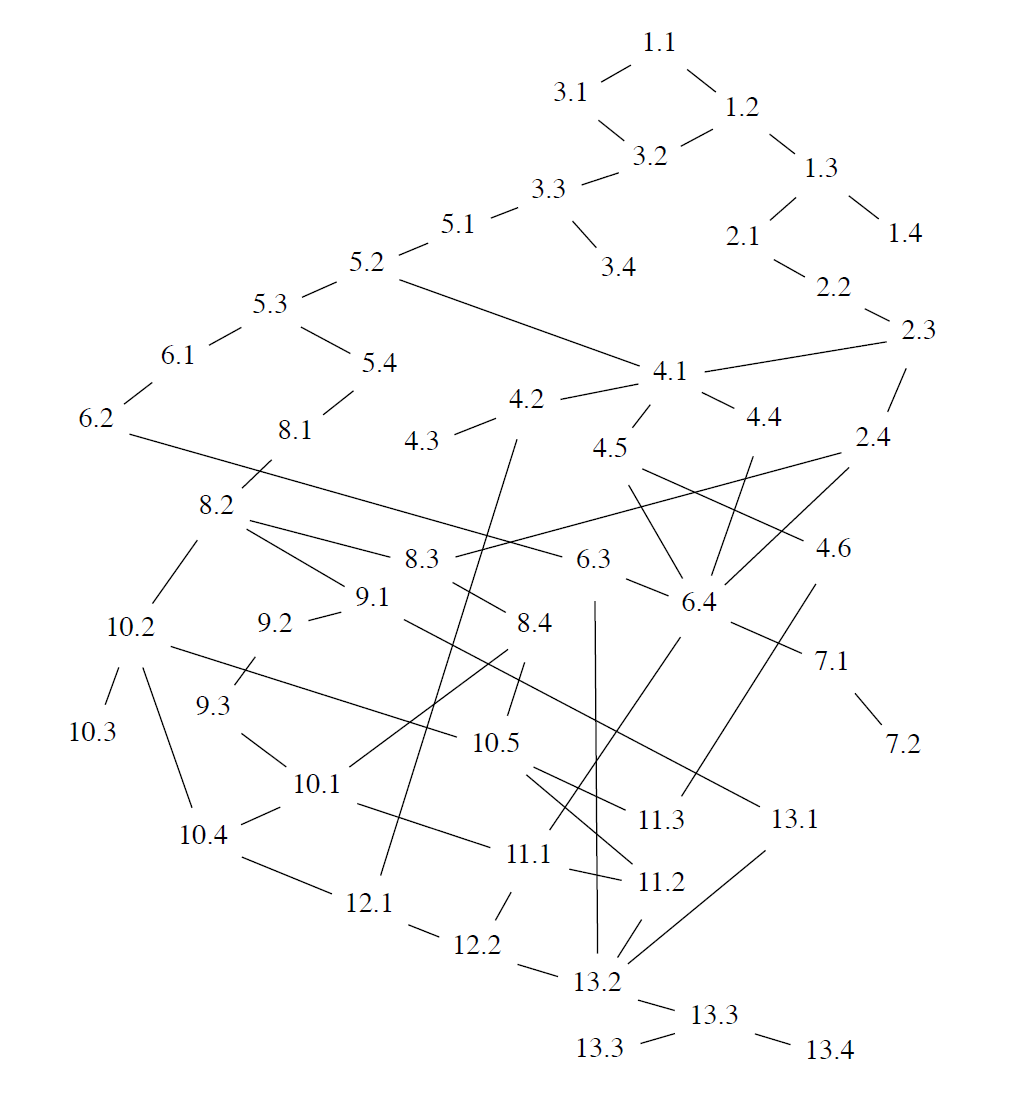
\includegraphics[width=.6\textwidth]{AoP_poset_of_section_dependencies} 
 \caption{"The partially ordered set of section dependencies" \parencite{beck_computing_2016}
\label{disciplinary_logic_LT_example}}
 \end{figure}
  
\begin{remark} Figure \ref{disciplinary_logic_LT_example} is an example that is self-contained and was not intended as an \gls{ltp} (since it was presented without instructional guides). Since the image is from a book on proofs meant to describe the logical, mathematical dependencies, this is genuinely a technical extreme version of a disciplinary-logic-and-cirricular-coherence approach to \gls{ltp}. \end{remark}

 
\subsubsection{Observable strategies and learning performances}
 
  Progress is described using observable behaviors, strategies or other learning performances, and each level is described using action verbs instead of mental conceptions.
  
\begin{multicols}{2}
\begin{itemize}
\item Features: Levels are organized using observable strategies or behaviors. There are differing assumptions in examples of \gls{ltp} written in this perspective about the connections between cognition and behavior.
\item Methods: Could be a product of research or informed by research.
\item Purpose: Communicating with teachers and teacher professional development. 
\item Benefits: Increase the precision and explicitness of \gls{ltp}, and help provide diagnostic or formative assessment information to teachers.
\item Trade-offs: Can miss out on details about conception/cognition. 
 \end{itemize}
 \end{multicols}
 
\subsubsection{Critiques of \gls{ltp} Research}

Diagnosing students and placing them in the appropriate level in an \gls{ltp} is not trivial. There are students who may appear to be on two different levels at the same time. Currently, the research in \gls{ltp} do adequately address the pressing issues of equity, diversity, race, language.

\end{document}
\end{document}
 

\newpage
\section{Fall 2019}

%---------------------------------------%
% Packages arranged by : Tsz Timmy Chan %
%                 Date : May 26th, 2019 % 
%---------------------------------------%

\documentclass{TC}
\usepackage{TCcommon}

\title{TITLE HERE}	% Work Title Here.
\author{Tsz Timmy Chan}	% YOUR NAME HERE 

\usepackage[notes]{TCheader}
\usepackage{TCexamtitle}

\usepackage{setspace}
\linespread{1.5}
\usepackage[acronym]{glossaries}

\makeglossaries
%\renewcommand{\benediction}{" " - }
%\renewcommand{\quoteoftheday}{" " \\ - }

\begin{document}


\subsection{Aug 26th---Aug 30th}	
	\subsubsection{LSRC 501: Introduction to the Course}
	
%---------------------------------------%
% Packages arranged by : Tsz Timmy Chan %
%                 Date : May 26th, 2019 % 
%---------------------------------------%

\documentclass{TC}
\usepackage{TCcommon}

\title{TITLE HERE}	% Work Title Here.
\author{Tsz Timmy Chan}	% YOUR NAME HERE 

\usepackage[notes]{TCheader}
\usepackage{TCexamtitle}

\usepackage{setspace}
\linespread{1.5}

%\renewcommand{\benediction}{" " - }
%\renewcommand{\quoteoftheday}{" " \\ - }

\begin{document}
Introduction: Emergence and development of the Learning Sciences

Read the work published in \gls{AERA} meant to give insight to the need for quality empirical research \parencite{noauthor_standards_2006}. 
Basically report all thinking, assume nothing - and be honest about particular methods used and any "massaging" the data.

\end{document}

	
	\subsubsection{LSRC 500: Introduction: Emergence and development of the Learning Sciences}	
	
%---------------------------------------%
% Packages arranged by : Tsz Timmy Chan %
%                 Date : May 26th, 2019 % 
%---------------------------------------%

\documentclass{TC}
\usepackage{TCcommon}

\title{TITLE HERE}	% Work Title Here.
\author{Tsz Timmy Chan}	% YOUR NAME HERE 

\usepackage[notes]{TCheader}
\usepackage{TCexamtitle}

\usepackage{setspace}
\linespread{1.5}

%\renewcommand{\benediction}{" " - }
%\renewcommand{\quoteoftheday}{" " \\ - }

\begin{document}
Reading about the pre-history and history of Learning Sciences. How did the field came to be separate from cognitive psychology, education, and other fields?

Made a timeline in class and spoke of the politics related to the founding of the young academic field of Learning Sciences \parencite{pea_prehistory_2016, kolodner_forward_2018, hoadley_short_2018}.
Some organizations, conferences and interests of note with respect to my interests:

\begin{itemize}
\item \gls{ICLS}
\item \gls{CSCL}
\item \gls{ACM}
\item \gls{AACE}
\item \gls{CSCW}
\item \gls{IRL}

\end{itemize}


\end{document}

	\subsubsection{DHD 510: An Introduction to Disability Studies Research Methodology}
	
%---------------------------------------%
% Packages arranged by : Tsz Timmy Chan %
%                 Date : May 26th, 2019 % 
%---------------------------------------%

\documentclass{TC}
\usepackage{TCcommon}

\title{TITLE HERE}	% Work Title Here.
\author{Tsz Timmy Chan}	% YOUR NAME HERE 

\usepackage[notes]{TCheader}
\usepackage{TCexamtitle}

\usepackage{setspace}
\linespread{1.5}

%\renewcommand{\benediction}{" " - }
%\renewcommand{\quoteoftheday}{" " \\ - }

\begin{document}
DHD 510: Got an intro to the field Disability Studies, defining the boundaries of the field with the relevant historical progression of the different conceptions of disability \parencite{linton_disability_1998, goodley_debates:_2011, edwards_disability_2003}. 

\end{document}

	
	
\subsection{Sept 2nd---Sept 6th}
	\subsubsection{LSRC 500: Theoretical perspectives and Frameworks on How People Learn: Cognitive, Cultural, Sociocultural, Communities of Practice.}
	
%---------------------------------------%
% Packages arranged by : Tsz Timmy Chan %
%                 Date : May 26th, 2019 % 
%---------------------------------------%

\documentclass{TC}
\usepackage{TCcommon}

\title{TITLE HERE}	% Work Title Here.
\author{Tsz Timmy Chan}	% YOUR NAME HERE 

\usepackage[notes]{TCheader}
\usepackage{TCexamtitle}

\usepackage{setspace}
\linespread{1.5}

%\renewcommand{\benediction}{" " - }
%\renewcommand{\quoteoftheday}{" " \\ - }

\begin{document}
Theoretical perspectives and Frameworks on How People Learn: Cognitive, Cultural, Sociocultural, Communities of Practice.

Examined the texts How People Learn 1 \& 2 and practiced comparing the two texts in more detail. Got an introduction to the differences between the cognitive and socioculture perspectives on learning and transfer \parencite{sawyer_learning_2014, satyam_cognitive_2018, national_academies_of_sciences_engineering_and_medicine_context_2018, national_academies_of_sciences_engineering_and_medicine_introduction_2018, national_research_council_design_1999,
national_research_council_learning:_1999}. Of particular interest is the diagram on perspectives on learning environments \ref{fig:NRC_perspectives_on_learning_enviornment}.

\begin{figure}[h]
\centering
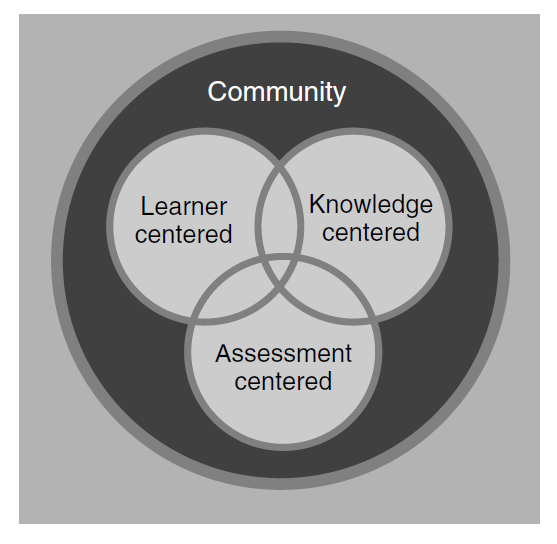
\includegraphics[width=.5\textwidth]{NRC_perspectives_on_learning_enviornment}

\caption{Perspectives on learning enviornments \parencite{national_research_council_design_1999}.}
\label{fig:NRC_perspectives_on_learning_enviornment}
\end{figure}

\end{document}

	
	\subsubsection{DHD 510: Conducting Research Overview}
	
%---------------------------------------%
% Packages arranged by : Tsz Timmy Chan %
%                 Date : May 26th, 2019 % 
%---------------------------------------%

\documentclass{TC}
\usepackage{TCcommon}

\title{TITLE HERE}	% Work Title Here.
\author{Tsz Timmy Chan}	% YOUR NAME HERE 

\usepackage[notes]{TCheader}
\usepackage{TCexamtitle}

\usepackage{setspace}
\linespread{1.5}

%\renewcommand{\benediction}{" " - }
%\renewcommand{\quoteoftheday}{" " \\ - }

\begin{document}
DHD 510: Conducting Research Overview

Basically read about the nature of scientific progress and revolutions, and what methodologies groups (quantitative and qualitative) are associated with particular epistemologies \parencite{titchkosky_introduction_2007, kuhn_progress_1996, sprague_field_2005, hahn_political_1993}. 

\end{document}

	
	\subsubsection{\gls{LSSA}: \gls{GSC} rep}
	Joined \gls{LSSA} and volunteered to become one of the \gls{GSC} representative.

\subsection{Sept 9th---Sept 13th}
	\subsubsection{LSRC 501: The Ongoing Debate about "Scientific" Research in Education}
	
%---------------------------------------%
% Packages arranged by : Tsz Timmy Chan %
%                 Date : May 26th, 2019 % 
%---------------------------------------%

\documentclass{TC}
\usepackage{TCcommon}

\title{TITLE HERE}	% Work Title Here.
\author{Tsz Timmy Chan}	% YOUR NAME HERE 

\usepackage[notes]{TCheader}
\usepackage{TCexamtitle}

\usepackage{setspace}
\linespread{1.5}

%\renewcommand{\benediction}{" " - }
%\renewcommand{\quoteoftheday}{" " \\ - }

\begin{document}
Snapshot of the current state of educational research, and what qualifies as scientific educational research?

"Debate" - can Educational Research be scientific? What is scientific?

Nice quotes:
"All models are wrong, some are useful" --- George Box\\
"Better an approximate answer to the right question than an accurate answer to the wrong question" --- John Tukey
Main Ideas and Takeaways on Feuer et al. ER Paper \parencite{feuer_scientific_2002}: 
	\begin{itemize}
	\item Developmental level of Education Research and its reputation - is this caused by funding, or the age of the field (immaturity)
	\item Science $\neq$ Methods
	\item Role of Government in Educational Research
	\item Culture relate to Education Research Quality; Self-Regulation
	\item Empiricism
	\item Similarity and difference between Education Research and other disciplines
	\item Multiple players $\implies$ multiple disciplines/bias/techniques
	\item Quantitative versus Qualitative Methods - $\exists$ tensions between folks who comes in with different "epidemiological baggage", and the inherent biases, leading to narrow views of what research is considered rigorous. "Educational research has a long history of struggling to become---or to ward off---science.
	\item Becomes a work on definition of \emph{rigor}.
	\item Educational research became a bit of a political 
	\item Science is often about measurement, and is dependent on the tools used to measure things. This means both physical tools as well as mathematics/statistics. 
	\item Science is not free from culture \& politics.
	\item contentions with the public opinion (inference: perhaps a harsher view Education due to personal experience, etc?)
	\end{itemize}




We also read the first 5 chapters of the NRC Report, and got some current understanding of the landscape of scientific educational research \parencite{national_research_council_introduction_2002, national_research_council_accumulation_2002, national_research_council_guiding_2002, national_research_council_features_2002, national_research_council_designs_2002}.

\begin{enumerate}[CH 1:]
\item Report Intro,
\item Accumulation of Knowledge,
\item Guiding Principles for Scientific Inquiry,
\item Features of Education and Educational Research,
\item Designs for the Conduct of Scientific Research in Education
\end{enumerate}
		\begin{itemize}
		\item Science is never finished, but improves warrants for knowledge over time
		\item Nature of progress is the same across fields = zigzagging paths. Progress is a function of time, money, and public support.
		\item Research-based knowledge in education has accumulated in this way, but Education = slower.
		\item 6 principles of Inquiry:
			\begin{enumerate}
			\item Significant questions that can be investigated empirically,
			\item Link research to relevant theory,
			\item Use methods that permit direct investigation of the question,
			\item Provide a coherent and explicit chain of reasoning,
			\item Replicate and generalize across studies,
			\item Disclose research to encourage professional scrutiny and critique. 
			\end{enumerate}
		\item Features of Education and the implications for inquiry
		\item Shelf life $\implies$ persistence?
		\item Ethics and designs for conducting research
		\item Three types of Education Research questions:
			\begin{enumerate}
			\item What's happening;
			\item Is there a systemic effect (casual effects?)
			\item How does it happen? (What is the underlying mechanism?)
			\end{enumerate}
		\end{itemize}
\begin{itemize}[(??)]
	\item Moderator vs Mediator definition between Treatments and Outcome.
\end{itemize}
\begin{itemize}[(!!)]
	\item Scientific $\subset$ Educational Research, but note that there exists valid scholarship that is $(\text{scientific})^c$.
	\item Consider \emph{who} wrote the literature, the \emph{intent} of the writer and people who commissioned the writing (be it publisher or government entity), and the \emph{audience} of the writer. 

\end{itemize}

\end{document}

	
	\subsubsection{LSRC 500: Cognitive and Sociocultural Perspectives on Learning and Transfer, Part 1}
	
%---------------------------------------%
% Packages arranged by : Tsz Timmy Chan %
%                 Date : May 26th, 2019 % 
%---------------------------------------%

\documentclass{TC}
\usepackage{TCcommon}

\title{TITLE HERE}	% Work Title Here.
\author{Tsz Timmy Chan}	% YOUR NAME HERE 

\usepackage[notes]{TCheader}
\usepackage{TCexamtitle}

\usepackage{setspace}
\linespread{1.5}

%\renewcommand{\benediction}{" " - }
%\renewcommand{\quoteoftheday}{" " \\ - }

\begin{document}


Went more into detail into cognitive and socioculture perspectives, and analyzed data from Dr. Allison Hall's work. Had a discussion on what we observed through the socio-cutulral lens and what we observed through the cognitive lens \parencite{j._pellegrino_perspectives_2012}.
\textit{(Feedback: My paper needs more operational definition with proper cititations, so that the critera used to determine what is cognitive and what is sociocultural will be more clear. Like Gubeladze said, papers need to be self-contained as much as possible!)}
\end{document}

	
	\subsubsection{DHD 510: Knowledge Produced About Disability vs. Disability Studies}
	
%---------------------------------------%
% Packages arranged by : Tsz Timmy Chan %
%                 Date : May 26th, 2019 % 
%---------------------------------------%

\documentclass{TC}
\usepackage{TCcommon}

\title{TITLE HERE}	% Work Title Here.
\author{Tsz Timmy Chan}	% YOUR NAME HERE 

\usepackage[notes]{TCheader}
\usepackage{TCexamtitle}

\usepackage{setspace}
\linespread{1.5}

%\renewcommand{\benediction}{" " - }
%\renewcommand{\quoteoftheday}{" " \\ - }

\begin{document}
Knowledge Produced About Disability vs. Disability Studies

Examined the growth and change in philosophy in methodologies, especially towards transdisciplinary ideals and emancipatory research \parencite{barnes_what_2003, kitchin_researched_2000, goodley_decolonizing_2012,
tregaskis_disability_2005}. 

When interviewing, especially with an \gls{intermediary}, it's important to conduct \gls{member checking}.

$\exists$ many instances of unethical and exploitative research where the researchers objectify those with disabilities and ignore the agency or boundaries of those with disabilities.

\begin{definition}[\Gls{reliability}]
\glsdesc{reliability}
\end{definition}
\begin{itemize}
\item Inter-rater or Inter-Observer: multiple observers to extract data or evaluate information, to make sure that the measure is objective by consensus. ($n \geq 3$ and $n$ should be odd).

\item Test-Retest: Give the test multiple times, it should give same results.

\item Parallel-Form: Same content, but different versions of the same test. 

\item Internal Consistency: Same question at different points to make sure that the response is consistent.  
\end{itemize}

\begin{definition}[\Gls{validity}]
\glsdesc{validity}
\end{definition}

\begin{itemize}
\item Internal Validity: The degree to which the results are associated with the independent variable; make sure that no other factors are affecting the outcomes

\item External Validity: Generalizability of the test across different studies

\item Construct Validity: The degree to which a test is actually measuring what it is intended to

\item Criterion-Related Validity: Is the research fitting pre-determined criterion?

\item Content Validity: Are the tests fitting the purpose of the research?

\item Ecological Validity: Is the research reflecting the world? (The setting chosen)
\end{itemize}


\vspace{-2em}
$$\text{Reliability}\equiv \text{Consistency (how far spread)} \;\; \text{Validity} \equiv  \text{Accuracy (how on target)} $$

\underline{\textit{Bias}}
Goal is to minimize bias (increase reliability/validity), and to do so one should learn to spot such bias in one's own and others' research.

\begin{itemize}
\item Sampling Bias: issues with choosing a sample that is not representative of the target population.

\item Selection Bias: Not randomly assigning folks between control/test groups. (Self-selection bias, where individuals choose to participate.)
\item Response Bias: People may give inaccurate answers because they are trying to give answers that they think the researcher wants to hear. (Yea-saying) Sometimes the researcher push until they get the answer they're looking for, or sometimes limit the research questions.
\item Hawthorne Effect: Some times the interaction with researchers can change the subjects' lifestyle; like if they have to keep track of their food/exercise, they may be a bit more "accountable". This can be moderated by control groups.  
\item Performance Bias: Researcher / participants are going to be changing their behavior based on their preconceived associations. Can be mediated by "blind" or "double blind" trials.	
\item Measurement Bias: people measuring or assessing the outcomes in a study should not know which individuals are in a test group or a control group.
\end{itemize}

Disability studies should benefit the people with disabilities and focus on removal of barriers in society. Power should be given to people with disability in creation of knowledge in disability studies. Research should include multitude of methods, so that we can give a more complete and complex view. 

Internalized ableism can be an influence on whether people identify as a disabled person. Not everyone who is disabled would identify as such, and this can introduce selection bias. 

Researchers have a platform, and thus a responsibility to collaborate with people with disabilities in giving voice to a marginalized community.
$$ \text{Inclusive research} = \text{Emancipatory} \cup \text{participatory research}$$

co-production is the outcome of1 participatory research.

Emancipatory research has the goal of empowerment, though transformation of the social dynamics of research; use the privilege of being a researcher to help remove barriers. 

Intersectional feminism and Queer/Crip approaches 

Participatory research: Empirical research that involves the participants in the decision making process. 

Action research: there should be an actionable outcome. 

Participatory Action Research (PAR): participation at each step of the research. 
Community Based Participatory Research (CBPR): Ecologically valid!

$CBPR \subset PAR$.


\end{document}



\subsection{Sept 16th---Sept 20th}
	\subsubsection{LSRC 501: Connecting Philosophy, Epistemology \& Methodology}
	
%---------------------------------------%
% Packages arranged by : Tsz Timmy Chan %
%                 Date : May 26th, 2019 % 
%---------------------------------------%

\documentclass{TC}
\usepackage{TCcommon}

\title{TITLE HERE}	% Work Title Here.
\author{Tsz Timmy Chan}	% YOUR NAME HERE 

\usepackage[notes]{TCheader}
\usepackage{TCexamtitle}

\usepackage{setspace}
\linespread{1.5}

%\renewcommand{\benediction}{" " - }
%\renewcommand{\quoteoftheday}{" " \\ - }

\begin{document}



Reading start to get a bit philosophical \parencite{bredo_philosophies_2006}.
	\begin{itemize}
		\item The author gave four ways of "getting to the bottom" of an idea :
			\begin{enumerate}
			\item "Method of tenacity": just hold your opinion really hard, which fails when your opponent is equally tenacious;
			\item "Method of authority": appeal to authority in a particular community, which fails when the authorities are not in agreement;
			\item "Method of a priori reasoning": finding underlying beliefs or assumptions that are common, which fails when the beliefs come from differently epistemologies,
			\item "Method of experiment": different epistemologies should be adopted as hypothetical and fallible, and tested in terms of their consequences. 			\end{enumerate}
		\item The author discussed the distinctions between \gls{externalist} and \gls{internalist} views, and the third, \gls{interactionism}, which is in between the two mentioned here.
		\item The thoughts leading up to post-positivism, post-modernism and critical theory.
		\item \Gls{externalist} thoughts $\implies$ \gls{empiricism} $\implies$ \gls{classicalpositivism} and  \gls{logicalpositivism}. Critiques of positivism that follow in succession of this line of \gls{externalist} school of thought thought are together taken as \gls{postpositivism}---though those who subscribe to postpositivism tend to still believe a model of research based on natural sciences, with the goals of searching for universal laws. This is in the left branch of \autoref{fig:green_philosophies}.
		\item Kantian rationalism is a critique of previous \gls{rationalism} on that it focuses too much on the mind (like Descartes, Spinoza and Leibniz) and also denounces the approach of \gls{empiricism} as focusing too little on the mind. 
		\item A tool that arose during the time of the development of these Romantic responses to Enlightenment \gls{empiricism} is \gls{hermeneutics}, which Dilthey (1833-1911) suggests that this methodological foundation provides a framework for cultural sciences distinct from natural sciences.
		\item \Gls{internalist} thoughts $\implies$ \gls{subjectiveidealism} $\implies$ \gls{structuralism}. Critiques of these eventually lead to \gls{postmodernism}; even structuralism has a given, where $\exists$ a structure at all. This is in the middle branch of \autoref{fig:green_philosophies}.
		\item \Gls{dialectic}al/Transactional Relation $\implies$ \gls{absoluteidealism} $\implies$ \gls{dialecticalmaterialism} $\implies$ \gls{criticaltheory} This is in the right-most branch of \autoref{fig:green_philosophies}.
		\item \Gls{criticaltheory} arose as a response to \gls{instrumentalrationality}
		\item And finally, standing on its own is\gls{pragmatism}, where local progress is possible without a notion of progress towards ultimate ends or directions. Truth is a matter of an idea's usefulness in guiding action. 
	\end{itemize}
	
	\begin{itemize}[(???)]
		\item What did the author mean when they said "Newton's explanation of planetary motion based on the law of gravitation really is correct, then empiricism \emph{must} be wrong because it cannot not account for such universal and necessary generalizations."?
	\end{itemize}
	\begin{itemize}[(!!!)]
	\item The text is indeed dense, but written in a way that is not conducive for reading by non-philosophers. In particular, the author chose to use words before they are well defined, and I believe the author did not do a good job at defining subjective idealism. 
	
	\item Similarly, transcendentalism was in the title of a section without once being defined.
	\item "knowing is primarily for the sake of action, and action changes what is known"
	\end{itemize}

\begin{figure}[h]
\centering
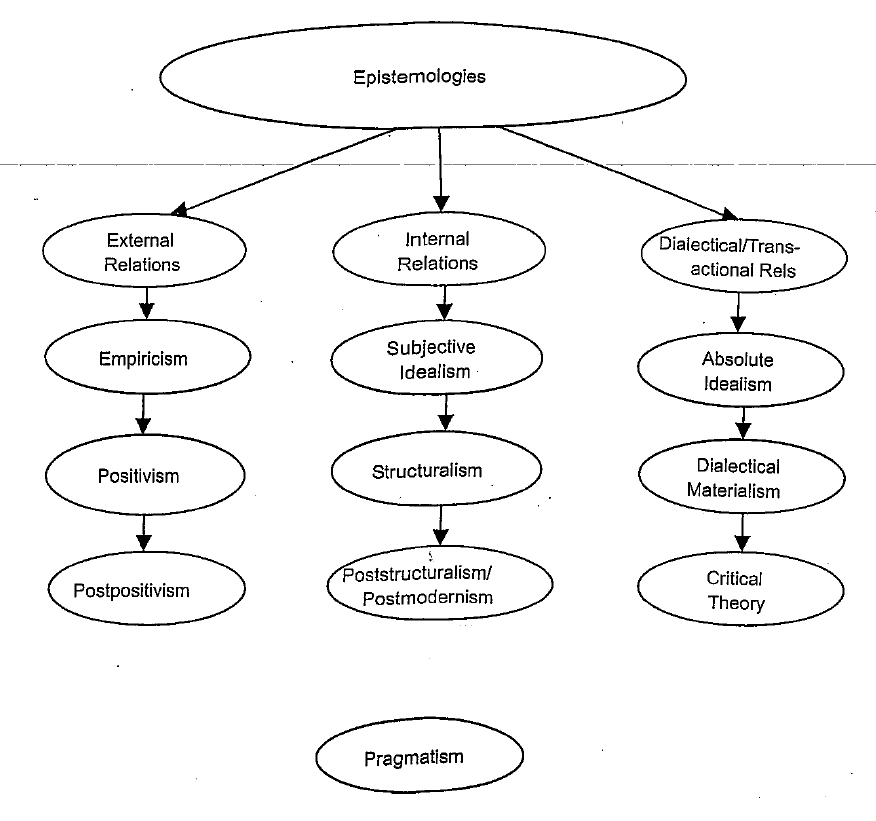
\includegraphics[width=.7\textwidth]{bredo_philosophies.png}
\caption{Arrangement of philosophies \parencite{bredo_philosophies_2006}}
\label{fig:green_philosophies}
\end{figure}
	
	\end{document}


	\subsubsection{LSRC 500: Cognitive and Sociocultural Perspectives on Learning and Transfer, Part 2}
	
%---------------------------------------%
% Packages arranged by : Tsz Timmy Chan %
%                 Date : May 26th, 2019 % 
%---------------------------------------%

\documentclass{TC}
\usepackage{TCcommon}

\title{TITLE HERE}	% Work Title Here.
\author{Tsz Timmy Chan}	% YOUR NAME HERE 

\usepackage[notes]{TCheader}
\usepackage{TCexamtitle}

\usepackage{setspace}
\linespread{1.5}

%\renewcommand{\benediction}{" " - }
%\renewcommand{\quoteoftheday}{" " \\ - }

\begin{document}


Discussed what makes an expert, how to become an expert, how to assist someone else to become an expert, and how to evaluate someone's expertise

Had a discussion on 
Discussed what is \gls{lpp}

Discourse of Gee:

Supplementary Readings, presented by Meerok and Erin:

\begin{itemize}
\item Primary discourse is what you grow up with at home and in families.
\item Secondary discourse arises when one leaves the primary discourse - and secondary first discusses those that involve print, but this also applies to film, TV, etc.
\item Acquisition vs Learning --- 
\end{itemize}  


\gls{ec} How people think about knowledge, what their beliefs are and how it manifests in their way of seeking knowledge. practices are a way to make beliefs about epistimic commitments visible - example, scientist will interrogate data. this way of studying actions reveal the beliefs underneath \parencite{fischer_epistemic_2018}:
\begin{itemize}
\item Features of LS research on \gls{ec}
	\begin{itemize}
	\item emphasizing multidisciplinary research
	\item broadening the range of questions
	\item challenging normative assumptions
	\item a focus on practices
	\item the throroughly social nature of \gls{ec},
	\item its situativity. 
	\end{itemize}
\end{itemize}
\begin{definition}[Epistemic practices]
Socially normed activites that people carry out accomplish epistemic aims such as developing evidence, arguments, theories and so on.
\end{definition}

C

\end{document}


	\subsubsection{DHD 510: Asking Research Questions from a Disability Studies Perspective}
	
%---------------------------------------%
% Packages arranged by : Tsz Timmy Chan %
%                 Date : May 26th, 2019 % 
%---------------------------------------%

\documentclass{TC}
\usepackage{TCcommon}

\title{TITLE HERE}	% Work Title Here.
\author{Tsz Timmy Chan}	% YOUR NAME HERE 

\usepackage[notes]{TCheader}
\usepackage{TCexamtitle}

\usepackage{setspace}
\linespread{1.5}

%\renewcommand{\benediction}{" " - }
%\renewcommand{\quoteoftheday}{" " \\ - }

\begin{document}
DHD 510: Research Questions

What makes good \emph{research} questions?
\begin{itemize}
\item Answerable
\item Significant (statistically)
\item Relevant to the disability community
\end{itemize}


Commitments:
\begin{itemize}
\item reflecting views \& experiences of those who are on the receiving end of policy \& practice

\item implication for to change

\item anti-ablist, anti-racist and anti-sexist
\end{itemize}

\gls{FINER}\parencite{cummings_conceiving_2007}
\begin{multicols}{2}
\begin{enumerate}
\item Feasible
	\begin{itemize}
	\item \# of participants
	\item technical expertise
	\item affordable (time \& \$\$)
	\item Manageable in scope 
	\end{itemize}
\item Interesting
	\begin{itemize}
	\item Investigator
	\item Peers
	\item Community
	\end{itemize}
\item Novel: Confirms/refutes or extends current research
\item Ethical: Make sure that study is amendable to review boards.
\item Relevant to
	\begin{itemize}
	\item scientific knowledge
	\item policy, practice and the real world
	\item future research
	\end{itemize}
\end{enumerate}
\end{multicols}

\gls{PICOT} \parencite{riva_what_2012}
\begin{enumerate}
\item Population: What specific population are you interested in learning about?
\item Investigation: What is your investigation? What will you be doing? Will you be surveying, observing, using video diaries? (Indicates methodologies)
\item Comparison Group: What is the main alternative group in contrast with the research population? (Some might not have one, if so you need to explain why.)

\item Outcome of Interest: What do you intend to accomplish, measure, improve or affect?
\item Time: What is the time-span that you will be looking at for your research? 
\end{enumerate}

\end{document}


	\subsubsection{Attended \gls{LSGSC}}
	Attended the \gls{LSGSC} of 2019 at Northwestern University on Sept $21^{\text{st}}$---$22^{\text{nd}}$, and volunteered for food preparation and I hope to become involved in the planning committee for next semester. 
	I attended a paper presentation session called "Embodied Technology in Science Learning", and a talk that really stood out for me was by \href{https://www.education.uw.edu/technologycenter/about-us/meet-the-staff/}{Erin Riesland from University of Washington}, and her email is \href{mailto:erinsage@uw.edu}{erinsage@uw.edu}. She mixed social sciences and VR!! How innovative and what a great perspective.
	
	
\subsection{Sept 23th---Sept 27th}
	\subsubsection{LSRC 501: Multiple Methods and a View on the History and Evolution of Learning Research}
	
%---------------------------------------%
% Packages arranged by : Tsz Timmy Chan %
%                 Date : May 26th, 2019 % 
%---------------------------------------%

\documentclass{TC}
\usepackage{TCcommon}

\title{TITLE HERE}	% Work Title Here.
\author{Tsz Timmy Chan}	% YOUR NAME HERE 

\usepackage[notes]{TCheader}
\usepackage{TCexamtitle}

\usepackage{setspace}
\linespread{1.5}

%\renewcommand{\benediction}{" " - }
%\renewcommand{\quoteoftheday}{" " \\ - }

\begin{document}
Then on the next chapter, it's a tiny bit more readable but still pretty dense, almost math textbook dense \parencite{green_epistemology_2006}.
	\begin{itemize}
	\item Pages on critiques of positivist focus, boiled down to...
		\begin{enumerate}
		\item Strong theory-dependence; i.e., observations, choices of procedures, and inferences made from data are dependent on the beliefs one holds about the world. Observations are not independent of the intellectual apparatus brought to bear on the objects of concern; finding observations that are truly indubitable was formidable, given variation in observer knowledge and perspective. 
		\item Data seem to underdetermine theory choice- there are instances in the history of science to suggest that multiple theories are equally supported by empirical evidence in a given instance.
		\item Any hypothesis is tested empirically, a number of auxiliary hypotheses are assumed at least provisionally true, and so that when a main hypothesis is tested and seemingly refuted, it may be due to an auxiliary hypothesis was mistakenly taken to be true when it was in fact false.
		\item Continual discovery of the social basis of disciplinary knowledge is in contradiction to the formalism of logical positivist epistemologies
		\item Plurality of knowledge systems is derived thru the work of particular epistemic communities.
		\end{enumerate}	
	\item $\exists$ multiple challenges to educational research:
		\begin{enumerate}
		\item Frustration with the degree and usefulness of knowledge relevant to education currently available
		\item Plurality has its advantages and should be encouraged, with a distinction between claims to validity (moral reasoning) and claims to truth (scientific reasoning).
		\end{enumerate}	
	\item One may address the above critiques and challenges through critical discourse, within group, regarding public reason and hermaneutical conversations across groups.
		\begin{enumerate}
		\item Within group --- Developmental and definitional work regarding the creation/specification/extension of research $\rightarrow$ theories, assumptions, ontological commitments. (include socialization of new members)
		\item With public reason --- Development of epistemological commitments to asses value of educational research across traditions $\rightarrow$ internal consistency, empricial adequacy, usefulness for practitioners
		\item Hermaneutics --- 
		\end{enumerate}
	\end{itemize}
	\begin{itemize}[(??)]
	\item Is this a version of pragmatism spoken of in Chapter 1?
	\end{itemize}

Smith Chapter on mixed methodologies \parencite{green_multiple_2006}: 
\begin{itemize}
\item Complex scenarios require mixed methodologies
\item $\exists$ different types and ways to use mixed methodologies
	\begin{enumerate}
	\item sequential design
	\item concurrent design
	\item confirmational
	\end{enumerate}
	
\item \gls{IES} goal structure
	\begin{enumerate}[\text{Goal} 1]
	\item Exploratory
	\item Development, usually uses \gls{dbr}
	\item Efficacy, usually uses \gls{rct} to demonstrate that under optimal conditions that $\exists$ effect
	\item Effectiveness: It worked, but can it be scaled? This is super expensive, typically over 10 million dollars, and most intervention inventions may end here.
	\end{enumerate}
\end{itemize}
Greeno Chapter in the same book \parencite{green_theoretical_2006}:

\begin{figure}[h]
\centering
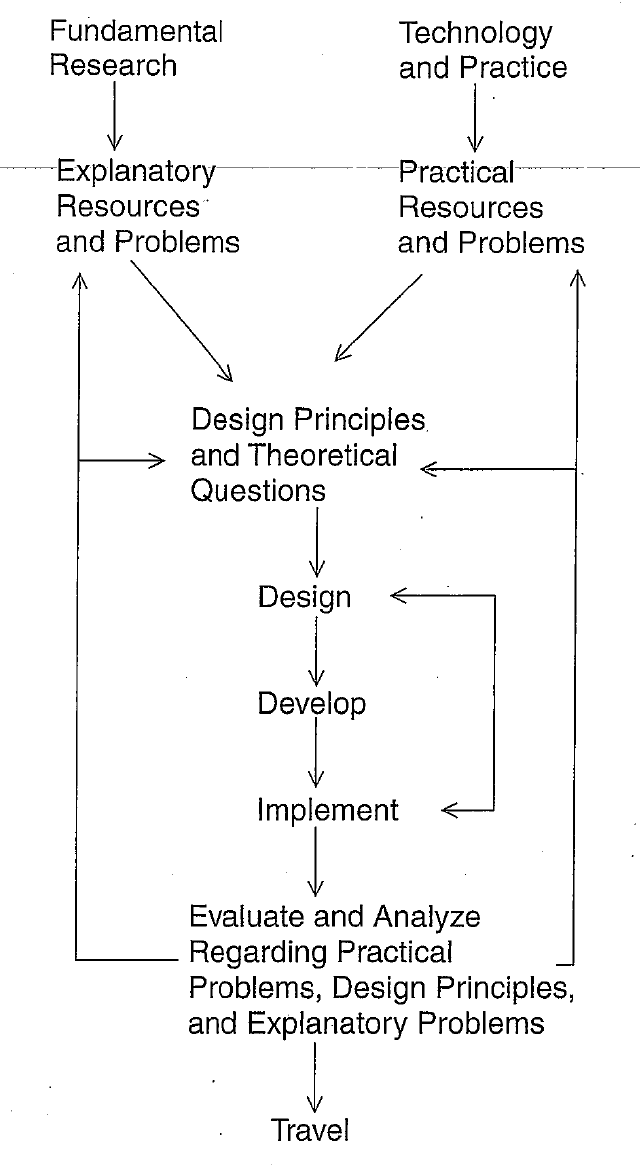
\includegraphics[width=.4\textwidth]{greeno_model_problem_solving_RandD.png}
\caption{Model of Problem Solving R \& D \parencite{green_theoretical_2006}}
\label{fig:Model_of Problem_Solving_R_and_D}
\end{figure}

\begin{itemize}
\item many discussions on the different types of methodologies, with some examples from the progress in math education.
\item Greeno defined design-based research as:

\begin{definition}[design-based research]
A view on research that understands fundamental research as a resource for design and development, includes attention to a body of design principles that can be developed in a field of engineering. See  \autoref{fig:Model_of Problem_Solving_R_and_D} for the pathways involved.
\end{definition}
\end{itemize}






\end{document}

	\subsubsection{\LaTeX\; workshop for \gls{LSSA}}
	Discussed with the Laura and Rubia about the creation of a workshop for \LaTeX. This means I'll begin writing material for an introductary course!
	
	\subsubsection{LSRC 500: Motivation, Self-regulation, and Metacognition}
	
%---------------------------------------%
% Packages arranged by : Tsz Timmy Chan %
%                 Date : May 26th, 2019 % 
%---------------------------------------%

\documentclass{TC}
\usepackage{TCcommon}

\title{TITLE HERE}	% Work Title Here.
\author{Tsz Timmy Chan}	% YOUR NAME HERE 

\usepackage[notes]{TCheader}
\usepackage{TCexamtitle}

\usepackage{setspace}
\linespread{1.5}

%\renewcommand{\benediction}{" " - }
%\renewcommand{\quoteoftheday}{" " \\ - }

\begin{document}


Chapter on Motivation, Engagement and Interest \parencite{fischer_motivation_2018}:
\begin{itemize}
\item Motivation is defined as follows 
\begin{definition}[Motivation]
(Engagement, Interest) $\in$ Motivation. Furthermore, $\exists$ more elements in this idea:
	\begin{multicols}{2}	
	\begin{itemize}
	\item perceptions/beliefs WRT achievement/ capability/competence
	\item expectancy
	\item value
	\item choice
	\item goals (short/long term)
	\item performance goal
	\item mastery goal
	\end{itemize}
	\end{multicols}
\end{definition}

\item Engagement
\item Interest
\end{itemize}

Chapter on Metacognition \parencite{sawyer_metacognition_2014}:
\begin{itemize}
\item Types of knowledge:
	\begin{itemize}
	\item 
	\end{itemize}
\end{itemize}

Chapter on Regulated Learning in Collaboration \parencite{fischer_contemporary_2018}: 

\end{document}

	
	\subsubsection{DHD 510: Reviewing Literature: Adding Disabled Voices}
	
%---------------------------------------%
% Packages arranged by : Tsz Timmy Chan %
%                 Date : May 26th, 2019 % 
%---------------------------------------%

\documentclass{TC}
\usepackage{TCcommon}

\title{TITLE HERE}	% Work Title Here.
\author{Tsz Timmy Chan}	% YOUR NAME HERE 

\usepackage[notes]{TCheader}
\usepackage{TCexamtitle}

\usepackage{setspace}
\linespread{1.5}

%\renewcommand{\benediction}{" " - }
%\renewcommand{\quoteoftheday}{" " \\ - }

\begin{document}
Conducting a Literature Review \parencite{alderman_conducting_2014}:
\begin{itemize}
\item Benefits of a literature review
	\begin{itemize}
	\item Assess current state of research
	\item Identify experts
	\item Identify key questions for further research
	\item Determine methodologies used in past studies of similar topics
	\end{itemize}
\item Steps to conduct a literature review
	\begin{enumerate}
	\item Selecting databases: use library discovery tools. 
		\begin{itemize}[\dangersign]
		\item Some database materials might not be included in discovery tool search
		\item No one tool does it all, "not even Google scholar"
		\item book collections might be excluded
		\item Features available in a particular database might not be available in a discovery tool.
		\item Some discovery tools limit results to what is available through a particular library's collections
		\item Review which databases have been included in the search, and which have not been included.
		\item Go \emph{backwards} by examining the articles in the bibliography to seek past articles, and go \emph{forward} by looking at the "Web of Science" and "Social Sciences Citation Index" to identify article citing the key articles identified in the previous steps \parencite{webster_analyzing_2002}. 
		\end{itemize} 
	\item Formulate an effective search strategy: know the field of that the database, as psychology terms may not work in a human resources management database. Use abstracts of relevant articles to build this list of search terms.
	\item Locate \textit{the actual items} and compose the review. End result should be to discuss the central themes in research and overview of significant studies.
	\item If the dissertation/thesis takes a long time to write, review the literature periodically.
	
	\end{enumerate}
\end{itemize}


\begin{figure}[h]

\begin{mdframed}
\centering
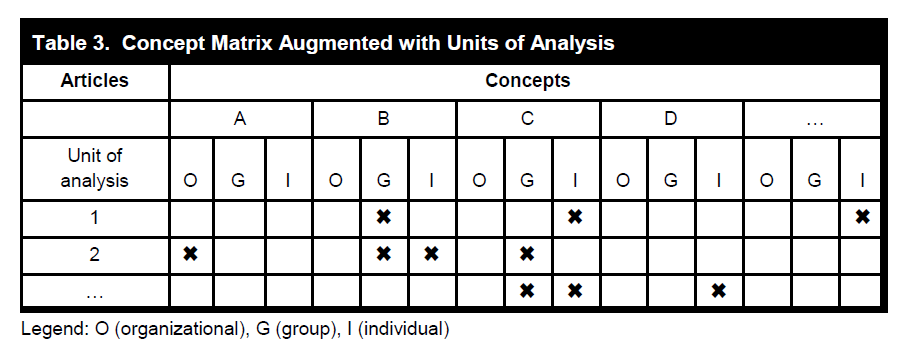
\includegraphics[width=.85\textwidth]{Author_to_Concept_Centric}
\end{mdframed}
\caption{Tool to move from author to concept centric organization \parencite{webster_analyzing_2002}.}\label{fig:Author_to_Concept_Centric}
\end{figure}


Writing a Literature Review \parencite{webster_analyzing_2002}:
\begin{itemize}
\item Types of literature review:
	\begin{enumerate}
	\item Mature topic where an accumulated body of research exists and require analysis and synthesis
	\item Emerging issue that would benefit from exposure to potential theoretical foundations.
	\end{enumerate}
\item Writing a Review Article
\begin{multicols}{2}
	\begin{enumerate}
	\item Beginning: 
		\begin{itemize}
		\item Hook your readers
		\item Provide working definition of key variables
		\item Articulate the paper's contributions such as:
			\begin{itemize}
			\item New theory to analyze or synthesize the existing literature
			\item Point out that little research currently exist
			\item Bring together previously-disparate streams of work
			\item Implications for practice
			\end{itemize}
		\item Identify the contexts in which the theory applies
		\item Support the scope of the search
		\end{itemize}
	\item Organize your literature: Move from author centric to concept centric. \dangersign Sometimes certain concepts are defined differently by different authors based on context or unit of analysis. See \autoref{fig:Author_to_Concept_Centric} for a tool to do such organization.
	\item Stylistics: 
		\begin{itemize}
		\item Tone: summary, so don't be overly critical  
		\item Tense: since this is about the state of the art, choose present tense. Unless you're attributing a concept to a specific person because that may change.
		\end{itemize}
	\item Guiding questions while writing:
		\begin{enumerate}
		\item What's new? (contribution)
		\item So what? (impact)
		\item Why so? (logic)
		\item Well done? (thoroughness)
		\end{enumerate}
	\end{enumerate}

\end{multicols}
\end{itemize}

Lecture Notes:
Types of literature review:
	\begin{itemize}
	\item Scoping (breadth): examining larger field of information.
	\item Rapid Evidence (depth): pick one issue of a part of an area.
	\item Systemic (breadth + depth): EVERYTHING that has been published on the topic. Usually begins with scoping, then identifies areas of focus and do a rapid evidence review on each focus.
		\begin{itemize}
		\item Narrative: Describe the data that is out there, usually as a first step to research projects.
		\item Analytic: Not just review, but also gives interpretation/theory. A good example is the "Who's Not Yet Here" article \parencite{burch_whos_2006}.
		\end{itemize}
	\end{itemize}
Parts of a literature review:
\begin{multicols}{2}
	\begin{itemize}
	\item Purpose
	\item Structure for searching.
		\begin{itemize}	
		\item Inclusion Criteria: "search parameters" to help structure the search and limit it to just relevant articles
			\begin{itemize}
			\item Location
			\item Time span
			\item Types of journals
			\item Databases
			\item Methodologies			
			\end{itemize}
		\item Keywords: most helpful words that are helpful, often the operational definitions; sometimes keywords differ based on time/location. (learning difficulties = UK; whereas intellectual disability = US after 2004, etc.) 
		\end{itemize}
	\item Search Strategy: have one, and know why you're doing this way.
		\begin{itemize}
		\item Boolean:
			\begin{itemize}
			\item uses logical operators \texttt{AND}, \texttt{OR}, \texttt{NOT}.
			\item Use quotes to define text phrases
			\item use asterisk (*) to search for the root of a word.
			\item Advanced search features help \emph{narrow} the search.
			\end{itemize}
		\item "Going backwards", look at the citations until \emph{point of saturation}, i.e., when you keep finding the same articles.
		\item "Go to the source" Begin with an expert - 
		\end{itemize}
	\end{itemize}
\end{multicols}
\textbf{GUIDELINES}
	\begin{multicols}{3}
	\begin{enumerate}
	\item Introduction
	\item Search structure
	\item Findings
	\item Discussion
	\item Conclusion
	\end{enumerate}
	\end{multicols}
Tips
	\begin{itemize}
	\item Pick a reference manager
	\item Choose a citation format
	\item Set up macro/keyboard shortcuts
	\end{itemize}
Theoretical / Conceptual Frameworks
	\begin{itemize}
	\item Theoretical framework explains how theory that is being used works with the research
	\item Helps organize ideas and explain \emph{how} particular frameworks are used.
	\item Operational definition sometimes come with a theoretical/conceptional framework
	\item Uusally in the background section, conception framework might come in during methods also
	\item Disciplinary background may lead to your theoretical framework
	\end{itemize}	

\end{document}

	
	
\subsection{Sept 30th---Oct 4th}
	\subsubsection{LSRC 500: Design and Support for Learning} 
	
%---------------------------------------%
% Packages arranged by : Tsz Timmy Chan %
%                 Date : May 26th, 2019 % 
%---------------------------------------%

\documentclass{TC}
\usepackage{TCcommon}

\title{TITLE HERE}	% Work Title Here.
\author{Tsz Timmy Chan}	% YOUR NAME HERE 

\usepackage[notes]{TCheader}
\usepackage{TCexamtitle}

\usepackage{setspace}
\linespread{1.5}

%\renewcommand{\benediction}{" " - }
%\renewcommand{\quoteoftheday}{" " \\ - }

\begin{document}
Scaffolding \parencite{sawyer_scaffolding_2014, fischer_research_2018} and Technology \parencite{sawyer_knowledge_2014}
\begin{itemize}
\item Work is shared between the learner and some more knowledgeable other or agent
\item Scaffolding enables the performance of a task more complex than the learner could handle alone, and enables learning from that experience.
\item \gls{zpd}: \glsdesc{gls-ZPD}
\item \gls{prolepsis}: \glsdesc{prolepsis}
\item As the learner appropriates this guidance and begin to regulate their own actions as the tutor gradually reduces guidance resulting in \emph{fading} of scaffolding
\item Scaffolding is more than just breaking down a problem into smaller sub-tasks (\textit{decomposition}); scaffolding is using a complex (expert level) task, which motivate developing subskills and requisite knowledge, applying knowledge and skill as they are \underline{constructed}.
\item scaffolding these aspects of work can make tasks tasks more productive for learning:
	\begin{enumerate}
	\item Sense-making: helping learners make sens of problems or data.
	\item Articulation \& reflection: helping learners articulate their thinking as they progress on problems
	\item Managing investigation \& problem-solving processes: helping learners with strategic choices and executing 
	\end{enumerate}
\item Possible benefits of scaffolding according to \parencite{sawyer_scaffolding_2014}:
	\begin{itemize}
	\item Simplifies elements of tasks so they are within reach of learners,
	\item Manage the process so learners can engage in elements of the disciplinary work in real problem contexts,
	\item Offset frustration and risk and maintain interest,
	\item Focus learners' attention on aspects of the problem they may take for granted,
	\item Prompt learners to explain and reflect,
	\item Enable learning by doing in context.
	\end{itemize}
\item According to there are three types of \gls{distributed scaffolding}: 
	\begin{itemize}
	\item \Gls{differentiated scaffolding}
	\item \Gls{redundant scaffolding}
	\item \Gls{synergistic scaffolding}
	\end{itemize}
\end{itemize}

Game based learning %\parencite{}

\end{document}

	
\subsection{Oct 7th---Oct 11th}
	\subsubsection{LSRC 501: Discourse I}
	
%---------------------------------------%
% Packages arranged by : Tsz Timmy Chan %
%                 Date : May 26th, 2019 % 
%---------------------------------------%

\documentclass{TC}
\usepackage{TCcommon}

\title{TITLE HERE}	% Work Title Here.
\author{Tsz Timmy Chan}	% YOUR NAME HERE 

\usepackage[notes]{TCheader}
\usepackage{TCexamtitle}

\usepackage{setspace}
\linespread{1.5}

%\renewcommand{\benediction}{" " - }
%\renewcommand{\quoteoftheday}{" " \\ - }

\begin{document}
Notes from Goldman Article:
\begin{itemize}
\item Discourse analysis of written text provides a method for systematically describing texts that students read as well as those they write. 

	
\begin{definition}[Readability]
	Reading difficulty of a passage, where traditional formulas fail to consider the familiarity of the concepts in the passage.
\end{definition}
\begin{definition}[Proposition (literacy research analysis)]
	Proposition is a theoretical unit of analysis that corresponds roughly to the meaning of a clause.  Propositions can be organized with propositional schemes and semantic networks.
\end{definition}

\begin{definition}[Predicate (literacy research analysis)]
Main verbs of clauses or connectives between clauses.
\end{definition}

\begin{definition}[Arguments (literacy research analysis)]
Arguments have functional roles WRT the predicate or can be embedded propositional schemes.
\end{definition}
\end{itemize}

\end{document}

	
	\subsubsection{DHD 510: Understanding and Evaluating Different Types of Research}
	
%---------------------------------------%
% Packages arranged by : Tsz Timmy Chan %
%                 Date : May 26th, 2019 % 
%---------------------------------------%

\documentclass{TC}
\usepackage{TCcommon}

\title{TITLE HERE}	% Work Title Here.
\author{Tsz Timmy Chan}	% YOUR NAME HERE 

\usepackage[notes]{TCheader}
\usepackage{TCexamtitle}

\usepackage{setspace}
\linespread{1.5}

%\renewcommand{\benediction}{" " - }
%\renewcommand{\quoteoftheday}{" " \\ - }

\begin{document}
Different disciplines have different established types of methods.

\begin{itemize}
\item Natural Sciences 
	\begin{itemize}
	\item Usually a quantitative approach
	\end{itemize}
\item Humanities
	\begin{itemize}
	\item Art, art history, music, philosophy, etc.
	\item Contrast with social sciences
	\item Significant overlap between social sciences \& humanities. 
	\item Not necessarily seeking to make claims -
	\item "What something is vs. the meaning we attach to it".	
		\begin{itemize}
		\item How disability has come to mean what it means,
		\item How those meanings come to be,
		\item How have the ways meaning been contested.
		\end{itemize}
	\item Critical \& Analytical
	\item "What does it mean to be human"?
	\item more \emph{philosophical} than social sciences
	\item within disabilities studies, the humanities perspective focuses on intersections with other critical fields with the purpose of social activism
	\item Struggle with the meaning of words---the way they are defined and recognize that words can be in flux and they are contextual.
	\item text can be data, where one can analyze the text itself.
	\item Some methods:
		\begin{itemize}
		\item Content Analysis
		\item \gls{CDA} --- this can be different between Humanities and Social Sciences! 
		\item Media
		\item LIteracy
		\item Art History, Art Production, etc.
		\end{itemize}
	\end{itemize}
\item Social Sciences
\end{itemize}


\textbf{types of research}
\begin{itemize}
\item Cross-sectional research: snapshot
\item Longitudinal research - over a length of time
\item Comparative research - comparison in the data, within group vs between group
\item intervention research - pre-post test design
\item Instrument development: new measure or adapting an existing one.
\item Evalutation research: formative vs summative  
\end{itemize}
\end{document}

	
\subsection{Oct 14th---Oct 18th}
	\subsubsection{LSRC 501: Discourse II}

	\subsubsection{LSRC 500: Technology in support of learning}
	Guest Speakers: Tom Moher, Joe Michaelis
	
%---------------------------------------%
% Packages arranged by : Tsz Timmy Chan %
%                 Date : May 26th, 2019 % 
%---------------------------------------%

\documentclass{TC}
\usepackage{TCcommon}

\title{TITLE HERE}	% Work Title Here.
\author{Tsz Timmy Chan}	% YOUR NAME HERE 

\usepackage[notes]{TCheader}
\usepackage{TCexamtitle}

\usepackage{setspace}
\linespread{1.5}

%\renewcommand{\benediction}{" " - }
%\renewcommand{\quoteoftheday}{" " \\ - }

\begin{document}

$\exists$ long list of possible educational technology, from paper/pencil $\to$ XR and machine learning tools.

Is a technology (method) in search of a problem, or problem in search of a technology(method)? (Should be the ladder).

Three articles:
\begin{itemize}
\item Classroom Orchestration: The Third Circle of Usability \parencite{dillenbourg_classroom_2011}
	\begin{itemize}
	\item
	\end{itemize}

\item Collective Inquiry in Communities of Learners \parencite{fischer_collective_2018}
\item Reading socially: Transforming the in-home reading experience with a learning-companion robot \parencite{michaelis_reading_2018}
	\begin{itemize}
	\item Why is the comparison to a paper based activity? What about other existing tech that can have that social element?
	\item Deep Understanding + Interest Development + Social Robotics 
	\end{itemize}
\end{itemize}

\end{document}

	\subsubsection{DHD 510}
	
%---------------------------------------%
% Packages arranged by : Tsz Timmy Chan %
%                 Date : May 26th, 2019 % 
%---------------------------------------%

\documentclass{TC}
\usepackage{TCcommon}

\title{TITLE HERE}	% Work Title Here.
\author{Tsz Timmy Chan}	% YOUR NAME HERE 

\usepackage[notes]{TCheader}
\usepackage{TCexamtitle}

\usepackage{setspace}
\linespread{1.5}

%\renewcommand{\benediction}{" " - }
%\renewcommand{\quoteoftheday}{" " \\ - }

\begin{document}

\begin{multicols}{2}

\begin{figure}[H]
\centering
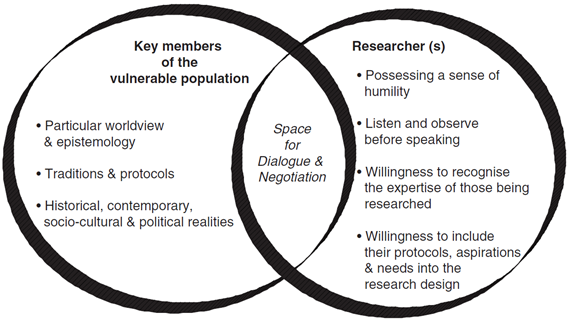
\includegraphics[width=.49\textwidth]{dialogue}
\caption{Creating the space for dialogue and negotiation}
\label{dialoguevulnerable}
\end{figure}
\begin{figure}[H]
\centering
\includegraphics[width=.49\textwidth]{power}
\caption{Power in Research with Vulnerable Populations}
\label{powervulnerable}
\end{figure}

\end{multicols}

Activity: Prisoners w/ mental illness - Perception of Authority
"Authority" - Remove CO's if possible
\begin{itemize}
\item Consent/Assent from guardian/CO/Wardens
\item Needs assessment: Medication, resource 
\item Compensation? 
\item create space to speak to prisoner alone if possible
\item remove identifiers from research if possible to avoid negative consequences for the participant
\item have a plan for crisis 
\item have a plan for lack of medicine or being forced to take medicine
\item have a plan for signs of retaliation from CO's and peers
\end{itemize}

\end{document}

	\subsubsection{LSRC 540: Tissenbaum}
	
%---------------------------------------%
% Packages arranged by : Tsz Timmy Chan %
%                 Date : May 26th, 2019 % 
%---------------------------------------%

\documentclass{TC}
\usepackage{TCcommon}

\title{TITLE HERE}	% Work Title Here.
\author{Tsz Timmy Chan}	% YOUR NAME HERE 

\usepackage[notes]{TCheader}
\usepackage{TCexamtitle}

\usepackage{setspace}
\linespread{1.5}

%\renewcommand{\benediction}{" " - }
%\renewcommand{\quoteoftheday}{" " \\ - }

\begin{document}
\Gls{DCLM} framework: understanding collaboration in open-ended tabletop learning environments 

\begin{itemize}
\item Contrasts with shared-goal collaboration, in an informal setting where participants walk in with different goals and get different things out of the environment.
\item Contrast with CLM / CCC where the state of communication $\equiv$ progress, where divergence is "poor collaboration"
\item 
\end{itemize}


\end{document}

	
\subsection{Oct 21st---Oct 25th}
	\subsubsection{LSRC 500: Mathematics Education}
	
%---------------------------------------%
% Packages arranged by : Tsz Timmy Chan %
%                 Date : May 26th, 2019 % 
%---------------------------------------%

\documentclass{TC}
\usepackage{TCcommon}

\title{TITLE HERE}	% Work Title Here.
\author{Tsz Timmy Chan}	% YOUR NAME HERE 

\usepackage[notes]{TCheader}
\usepackage{TCexamtitle}

\usepackage{setspace}
\linespread{1.5}

%\renewcommand{\benediction}{" " - }
%\renewcommand{\quoteoftheday}{" " \\ - }

\begin{document}
Ball paper: \gls{MKT} 
\begin{itemize}
\item \gls{CCK}
\item \gls{SCK}
\item Horizon
\item \gls{KCT}
\item \gls{KCS}
\item Curriculum
\end{itemize}

\end{document}

	\subsubsection{DHD 510: Research Methods, Quantitative}
	
%---------------------------------------%
% Packages arranged by : Tsz Timmy Chan %
%                 Date : May 26th, 2019 % 
%---------------------------------------%

\documentclass{TC}
\usepackage{TCcommon}

\title{TITLE HERE}	% Work Title Here.
\author{Tsz Timmy Chan}	% YOUR NAME HERE 

\usepackage[notes]{TCheader}
\usepackage{TCexamtitle}

\usepackage{setspace}
\linespread{1.5}

%\renewcommand{\benediction}{" " - }
%\renewcommand{\quoteoftheday}{" " \\ - }

\begin{document}
Types of Variables

\begin{itemize}
\item Independent / Dependent / Controlled
\item Examples of statistical data: SPSS, SAS, STATA
\item Continuous vs Discrete: Uncountable vs Countable 

\item Types of Experimental \& Quasi-experimental design
	\begin{itemize}
	\item  Post Test Only
	\item Pre-post test
	\item Soloman Four: Usually used when one is not certain if pretest influences treatment.\\
		\begin{tabular}{c|c|c|c}
			& Pretest & Treatment & Posttest \\
		Treatment & 1 & 1 & 1 \\
		Control & 1 & 0 & 1 \\
		Treatment & 0 & 1 & 1 \\
		Control & 0 & 0 & 1
		\end{tabular}
	\end{itemize}
\end{itemize}

\end{document}

	
\subsection{Oct 28th---Nov 1st}
	\subsubsection{DHD 510: Research Methods, Qualitative}
	%---------------------------------------%
% Packages arranged by : Tsz Timmy Chan %
%                 Date : May 26th, 2019 % 
%---------------------------------------%

\documentclass{TC}
\usepackage{TCcommon}

\title{TITLE HERE}	% Work Title Here.
\author{Tsz Timmy Chan}	% YOUR NAME HERE 

\usepackage[notes]{TCheader}
\usepackage{TCexamtitle}

\usepackage{setspace}
\linespread{1.5}

%\renewcommand{\benediction}{" " - }
%\renewcommand{\quoteoftheday}{" " \\ - }

\begin{document}

Qualitative Research Traditions:
\begin{itemize}
\item Narrative Inquiry: Biography, autobiography, life history and oral history. Mainly uses interviews and primary documents. Looking for epiphanies, and examines context. \emph{Outcome: Detailed picture of an individual's life.} 
\item Phenomenology: "Pre-sociology" often used by philosophy. Long interviews with $\approx 10$ people. Examines statements, meanings, meaning themes, general descriptions of the experience. \emph{Outcome: "Essence" of the experience.}
\item Grounded Theory: produce a theory/model (Very structured) Interview with 20-30 people. Uses the techniques: Open coding, Axial coding, Selective coding, Conditional matrix. \textit{Outcome: theory \& theoretical model}
\item Ethnography: comes from anthropology - describing a culture and social group. Examines observations, interviews and other artifacts and often immersion over a long time. Analysis done using description and interpretation. \emph{Outcome: description of the culture behavior of a group or an individual.}
\item Case Study: In-depth study of a particular "case". Multiple sources - documents, archival records, interviews, observations, physical artifacts. Analysis: Description, themes, assertions.
\end{itemize}

Qualitative Methods:
\begin{itemize}
\item Document and Archival Analysis: document = data.
\item Observation: systematically taking notes \& recording in naturalistic setting.  
\item Interview: interaction based, one-on-one.
\item Focus Groups: group interviews. Used when one-on-one is limiting. 
\end{itemize}


Qualitative Sampling Strategies (instead of random...):
\begin{itemize}

\item Maximal variation sampling (every category represented)
\item Extreme case sampling (get outlier; extreme characteristics) 
\item Theory/concept sampling (fits operational definition)
\item Homogeneous sampling (something in common)
\item Critical Sampling (challenging a phenomenon)
\item Opportunistic/emergent sampling (due to unfolding events) \textit{This is different from Convenient sampling!}
\item Snowball Sampling (ask participants to refer others)
\end{itemize}


$$(\textbf{Trustworthiness, Rigor}) \simeq (\textbf{Reliability, Validity)}$$

Trustworthiness:
\begin{enumerate}
\item Credibility
\item Transfer-ability
\item Dependability
\item Confirm-ability 
\end{enumerate}

TRIANGULATION \& MEMBER CHECKING are gold standards, because they theoretically should increase the 



\end{document}

	
\subsection{Nov 4th---Nov 8th}
	\subsubsection{DHD 510: Observation}
	
%---------------------------------------%
% Packages arranged by : Tsz Timmy Chan %
%                 Date : May 26th, 2019 % 
%---------------------------------------%

\documentclass{TC}
\usepackage{TCcommon}

\title{TITLE HERE}	% Work Title Here.
\author{Tsz Timmy Chan}	% YOUR NAME HERE 

\usepackage[notes]{TCheader}
\usepackage{TCexamtitle}

\usepackage{setspace}
\linespread{1.5}

%\renewcommand{\benediction}{" " - }
%\renewcommand{\quoteoftheday}{" " \\ - }

\begin{document}
\begin{definition}[\gls{thick description}]
\glsdesc{thick description}
\end{definition}

\begin{definition}[\gls{naturalistic observation}]
\glsdesc{naturalistic observation}]
\end{definition}

EMIC
Insider perspective (local) - observes behavior within a group, culture, or organization.

\begin{tabular}{p{.75in}|p{2.25in}|p{2.25in}}
& Pros & Cons \\ \hline
EMIC & 
\begin{minipage}{2in}

\begin{itemize}
\item Understand the POV from other cultures
\item What is important and meaning to those within group
\item in depth, rich and holistic knowledge
\end{itemize}
\end{minipage}
&
\begin{minipage}{2in}
\begin{itemize}
\item Difficult to make comparison
\item Researcher subjective bias
\item Research can take more resources 
\end{itemize}
\end{minipage} \\ \hline

ETIC & 

\begin{minipage}{2in}
\begin{itemize}
\item Allows comparison between cultures
\item Researcher decides what is important before hand
\item Multiple cultures can be observed at once
\end{itemize}
\end{minipage} & 

\begin{minipage}{2in}
\begin{itemize}
\item 
\end{itemize}
\end{minipage}

\end{tabular}

\end{document}

	
\subsection{Nov 11th---Nov 15th}

\subsection{Nov 18---Nov 22nd}
	\subsubsection{DHD 510: Data Analysis}
	
%---------------------------------------%
% Packages arranged by : Tsz Timmy Chan %
%                 Date : May 26th, 2019 % 
%---------------------------------------%

\documentclass{TC}
\usepackage{TCcommon}

\title{TITLE HERE}	% Work Title Here.
\author{Tsz Timmy Chan}	% YOUR NAME HERE 

\usepackage[notes]{TCheader}
\usepackage{TCexamtitle}

\usepackage{setspace}
\linespread{1.5}

%\renewcommand{\benediction}{" " - }
%\renewcommand{\quoteoftheday}{" " \\ - }

\begin{document}
\begin{itemize}
\item Statistical Analysis
	
	\begin{itemize}
		\item Descriptive statistics are not analysis
		\item Parametric VS. Nonparametric
			\begin{itemize}
			\item Parametric analysis to test group \emph{means}; assumes normality, homogeneity of variances, and independence.
			\item Nonparametric analysis to test medians:
			Used when data does not meet the assumptions required for parametric tests - usually when mean and median do not line up.
			\end{itemize}
	\end{itemize}
	\begin{itemize}
	\item Variance Analysis
		\begin{itemize}
		\item t-tests
		\item One-way ANOVA
		\item One way repeated measures ANOVA
		\item Factorial ANOVA
		\item ANCOVA: Analysis of co-variance.
		\item MANOVA: Multiple dependent variables 
		\end{itemize}
	\item Correlational Analysis
		\begin{itemize}
		\item Pearson Correlation---tests for strength of the association of two continuous variables
		\item Spearman Correlation---Tests for the strength of the association between two ordinal variables.
		\item Chi-Squared---Tests for the strength of the association between two categorical variables
		\end{itemize}
	\item Regression Analysis
		\begin{itemize}
		\item Simple Linear Regression---Tests how change in the predictor variable predicts 
		\item Multiple Regression---Linear but high dimensional.
		\end{itemize}
	\end{itemize}
\item Qualitative Coding \& Codebooks	
	\begin{itemize}
	\item Codebook for analysis:
		\begin{itemize}
		\item In qualitative research, a codebook is a set of codes and definitions used as a guide to help when doing analysis
		\item Codes are used to categorize verbatim quations from research participants
		\end{itemize}
	\item Software for qualitative analysis includes ATLAS.ti and NVivo
		\begin{itemize}
		\item Software = more efficient when collaborating
		\item ppl still do this by hand tho cuz it's more "involved"
		\item coding becomes a way to become immersed in the data
		\end{itemize}
	\item Index coding: develop an index of code a priori.
	\item Thematic Coding: create codes that capture core themes that emerge in the research
	\item Grounded Theory: 
		\begin{enumerate}
		\item Open Coding---form initial categories about the phenomenon 
		\item Axial Coding---Assemble data in new ways after open coding 
		\item Selective Coding---identify a storyline and write a story that integrates categories from axial coding
		\end{enumerate}
	\end{itemize}
\item Quantitative Analysis: Deductive (theory driven) and inductive (emerges through data)
	\begin{itemize}
	\item Content analysis---conceptual/relational analysis to understand the actual content and internal features of media
	\item Discourse analysis---linguistic analysis of ongoing flow of communication, looking at verbal and non-verbal communications.
	\item Constant comparison/Grounded Theory---Each interpretation/finding is compared with existing findings as they emerge
	\item Thematic analysis---looks for themes
	\item Narrative Analysis---Focuses on the way people make/use stories to interpret the world around them (structural/functional approach or sociology of stories)
	\item Hermaneutical Analysis---Methodology of interpretation; problems that arise when dealing with meaningful human actions and the products of such actions, most importantly texts.
	\item Phenomenological/Heuristic Analysis===The study of how individuals experience the world. 
	\end{itemize}
\end{itemize}
\end{document}

\end{document}



\newpage

\printbibliography[heading=bibintoc]


\newpage
\printglossary[type=\acronymtype]
\printglossary





\end{document}
